\documentclass[oneside,a4paper,12pt]{article}
\usepackage{graphicx}
\usepackage{amsmath}
\usepackage{listings}
\graphicspath{{~/templates/}, {../images/}}

\makeindex
\begin{document}
	\begin{titlepage}
		\includegraphics[width=4cm]{logopopo.png}
		\hspace*{\fill}
		\includegraphics[width=6cm]{logouniv.png}
		
		\begin{center}
			\vspace{1cm}
			\textbf{TP Support de Transmission}\\
			\textbf{Mélageur à diode}\\
			\vspace{1cm}
			\textbf{Maxence LAURENT, Thibault VOLLERIN, Maxence NEUS}\\
			\vspace{3cm}
			%\includegraphics[width=13cm]{titlepage.png}\\
			\vspace{\fill}
			\textbf{Mars 2022}\\
		\end{center}
	\end{titlepage}
	
	\tableofcontents
	
	\vspace{5cm}
	
	\begin{abstract}
	
 	\end{abstract}

	\newpage

	\section{Préparation}
	
	\newpage

	\section{Manipulations}

	\subsection{Etalonage}

	Il est nécessaire de calibrer les atténuateurs pour connaître la puissance injectée au mélangeur.
	Pour cela on fait varier la valeur de l'atténuateur pour avoir une puissance prédéfini à l'entrée du mélangeur.
	
	\subsection{Isolations}

	On visualise le spectre de puissance en voie IF autour des fréquences $f_{RF}$ et $f_{OL}$:

	\begin{figure}[h]
		\centering
		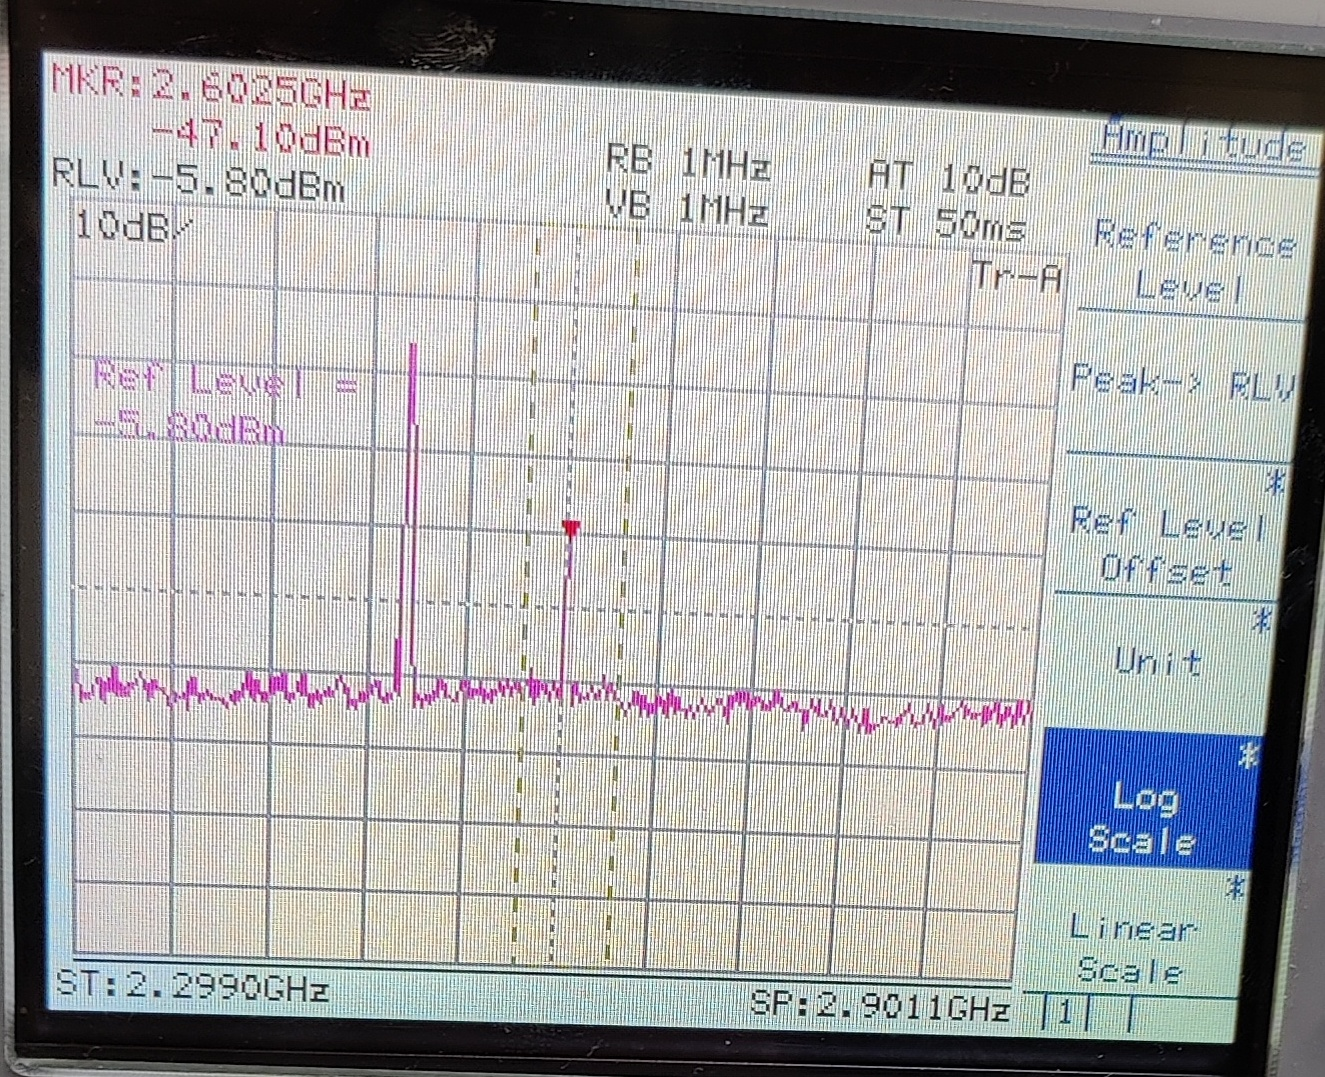
\includegraphics[width=8cm]{manip1.jpg}	
		\caption{Raies en voie IF}
	\end{figure}

	On a mesuré les puissances des raies :
	\[ P_{OL}(IF) = -22dBm \]
	\[ P_{RF}(IF) = -47dBm \]

	On en déduit les isolations:
	\[ I_{RF_IF} = P_{RF}(RF) - P_{RF}(IF) = (-20 dBm) - (-47 dBm) \]
	\[ I_{RF_IF} = 27 dB \]

	\[ I_{OL_IF} = P_{OL}(OL) - P_{OL}(IF) = (7 dBm) - (-22 dBm) \]
	\[ I_{OL_IF} = 29 dB \]

	\newpage

	\subsection{Pertes de conversion}

	On a mesuré la puissance à $f = f_{RF}-f_{OL}$ pour déterminer les pertes de convertion :
	\[ P_{RF}(RF) - P_{RF-OL}(IF)  \]

	\begin{figure}[h]
		\centering
		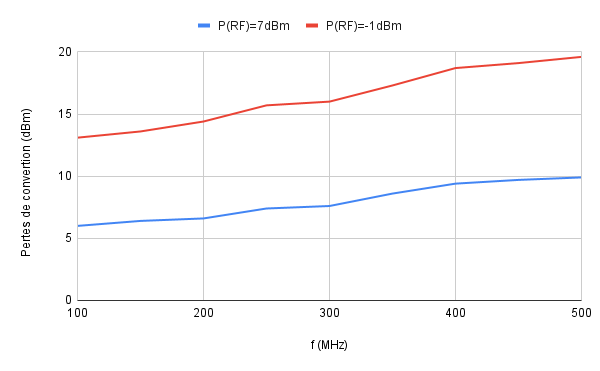
\includegraphics[width=10cm]{pertesfIF.png}	
		\caption{Pertes de convertions en fonction de $f_{IF}$}
	\end{figure}

	On voit que comme indiqué sur la datasheet, les pertes en convertion sont constantes pour $f_{RF}$ à 200MHz autour de $f_{OL}$.
	
	\begin{figure}[h]
		\centering
		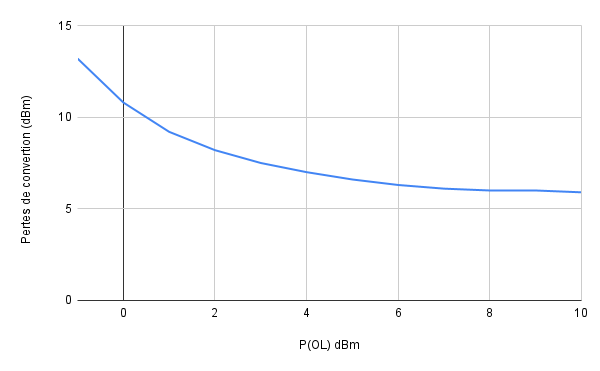
\includegraphics[width=10cm]{manip2.png}	
		\caption{Pertes de convertions en fonction de $P_{OL}$}
	\end{figure}

	On observe que les pertes de convertion décroissent quand $P_{OL}$ augmente, en effet plus $P_{OL}$ est grand,
	plus le mélangeur oppère dans une plage non linéaire et est donc plus efficace.

	\begin{figure}[h]
		\centering
		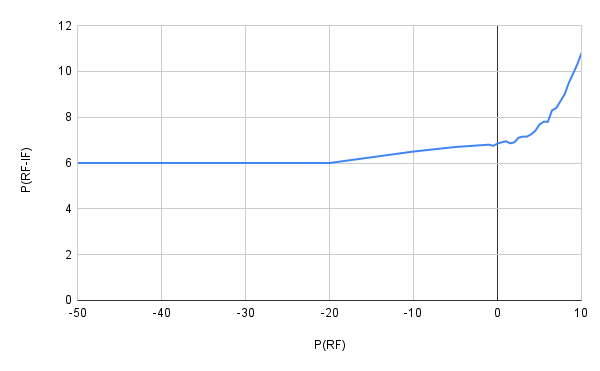
\includegraphics[width=10cm]{ptCompression.png}	
		\caption{Pertes de convertions en fonction de $P_{RF}$}
	\end{figure}

	Le point de compression correspond au point tel que les pertes de convertion se dégradent de 1dB. 
	Ici on voit sur le graph que ce point se trouve autour de $P_{RF}=0dBm$. Avant ce point, les pertes sont constantes autour de 6dB.

	\begin{figure}[h]
		\centering
		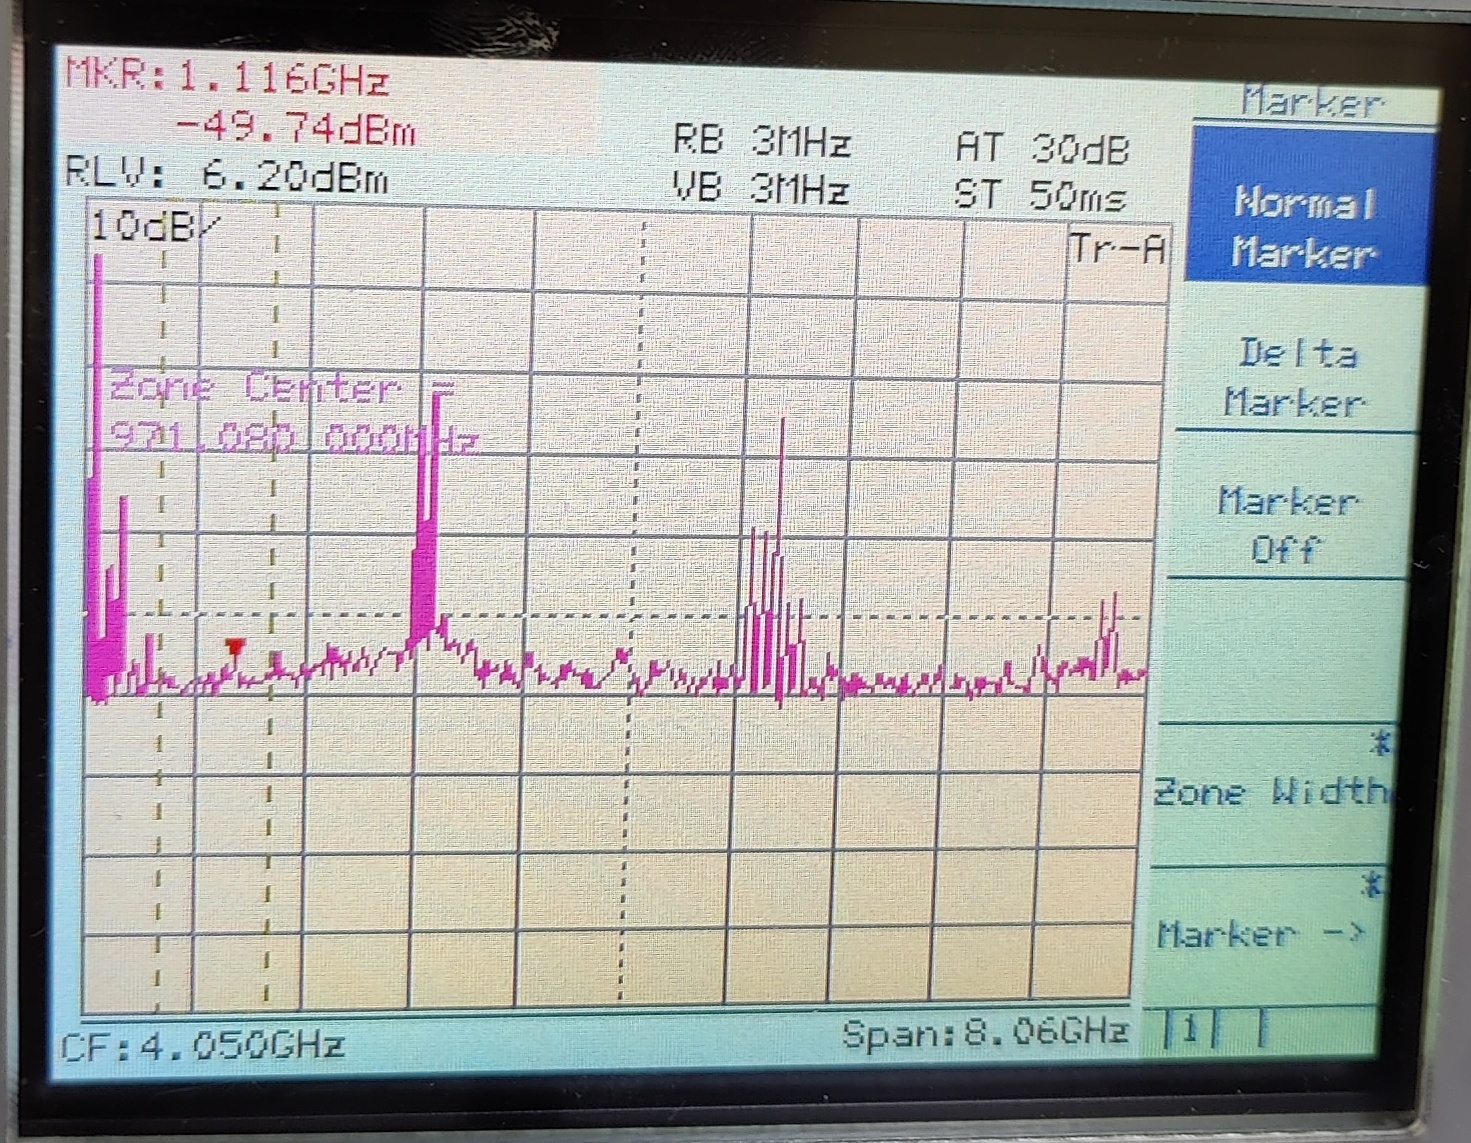
\includegraphics[width=9cm]{manip4.jpg}	
		\caption{Spectre complet en voie IF à $P_{RF} = 10dBm$}
	\end{figure}

	\newpage
	\section{Conclusion}

\end{document}
